\documentclass[twoside, 11pt]{article}
\usepackage{biblatex} %Imports biblatex package
\addbibresource{snake.bib}
\usepackage{blindtext} % Package to generate dummy text throughout this template 
\usepackage{amsmath}
\usepackage[sc]{mathpazo} % Use the Palatino font
\usepackage[T1]{fontenc} % Use 8-bit encoding that has 256 glyphs
\linespread{1.00} % Line spacing - Palatino needs more space between lines
\usepackage{microtype} % Slightly tweak font spacing for aesthetics

\usepackage[english]{babel} % Language hyphenation and typographical rules
\usepackage{geometry} % Document margins
\geometry{
  paper=letterpaper,
  margin=1in,
}
\usepackage[hang, small,labelfont=bf,up,textfont=it,up]{caption} % Custom captions under/above floats in tables or figures
\usepackage{booktabs} % Horizontal rules in tables

\usepackage{lettrine} % The lettrine is the first enlarged letter at the beginning of the text

\usepackage{enumitem} % Customized lists
\setlist[itemize]{noitemsep} % Make itemize lists more compact
\usepackage{graphicx}
\usepackage{graphbox}
\usepackage{abstract} % Allows abstract customization
\renewcommand{\abstractnamefont}{\normalfont\bfseries} % Set the "Abstract" text to bold
\renewcommand{\abstracttextfont}{\normalfont\small\itshape} % Set the abstract itself to small italic text

\usepackage{titlesec} % Allows customization of titles
\renewcommand\thesection{\Roman{section}} % Roman numerals for the sections
\renewcommand\thesubsection{\roman{subsection}} % roman numerals for subsections
\titleformat{\section}[block]{\large\scshape\centering}{\thesection.}{1em}{} % Change the look of the section titles
\titleformat{\subsection}[block]{\large}{\thesubsection.}{1em}{} % Change the look of the section titles

\usepackage{fancyhdr} % Headers and footers
\pagestyle{fancy} % All pages have headers and footers
\fancyhead{} % Blank out the default header
\fancyfoot{} % Blank out the default footer
\fancyhead[C]{Modular Soft Snake Robot $\bullet$ November 2022} % Custom header text
\fancyfoot[RO,LE]{\thepage} % Custom footer text
\usepackage{titling} % Customizing the title section
\usepackage{textcomp, gensymb}
\usepackage{subcaption}
\usepackage{float}

\usepackage{tikz}
\usetikzlibrary{shapes.geometric, arrows, chains}

\tikzstyle{startstop} = [rectangle, rounded corners, 
minimum width=2cm, 
minimum height=1cm,
text centered, 
draw=black, 
fill=red!30]

\tikzstyle{coord} = [
coordinate, 
node distance=2cm
]

\tikzstyle{io} = [trapezium, 
trapezium stretches=true, % A later addition
trapezium left angle=70, 
trapezium right angle=110, 
minimum width=1cm, 
minimum height=1cm, text centered, 
text width=1.5cm,
draw=black, fill=blue!30]

\tikzstyle{process} = [rectangle, 
minimum width=1cm, 
minimum height=1cm, 
text centered, 
text width=3cm,
draw=black, 
fill=orange!30]

\tikzstyle{decision} = [diamond, 
minimum width=1cm, 
minimum height=1cm, 
text centered, 
aspect=2,
draw=black, 
text width=1.5cm,
fill=green!30]

\tikzstyle{arrow} = [thick,->,>=stealth]
\usepackage[colorinlistoftodos]{todonotes}
\usepackage{hyperref} % For hyperlinks in the PDF
\graphicspath{{images/}}
\counterwithin{figure}{section}
\renewcommand{\thefigure}{\arabic{section}.\arabic{figure}}
\usepackage{parskip}
\counterwithin{table}{section}
\renewcommand{\thetable}{\arabic{section}.\arabic{table}}
\usepackage{pgfplots}
\usepackage{titlesec}
\usepackage{verbatim}
\pgfplotsset{compat=1.11}
%----------------------------------------------------------------------------------------
%	TITLE SECTION
%----------------------------------------------------------------------------------------

%\setlength{\droptitle}{-4\baselineskip} % Move the title up

%\pretitle{\begin{center}\Huge\bfseries} % Article title formatting
%\posttitle{\end{center}} % Article title closing formatting
%\title{Research on a multi-degree-of-freedom modular soft snake robot} % Article title
%\author{%
%\textsc{Hongyi Hu} \\[1ex] % Your name
%\normalsize The Overlake School \\ % Your institution
%\normalsize \href{mailto:ethanhu8351@gmail.com}{ethanhu8351@gmail.com} % Your email address
%\and % Uncomment if 2 authors are required, duplicate these 4 lines if more
%\textsc{Jane Smith}\thanks{Corresponding author} \\[1ex] % Second author's name
%\normalsize University of Utah \\ % Second author's institution
%\normalsize \href{mailto:jane@smith.com}{jane@smith.com} % Second author's email address
%}
%\date{\today} % Leave empty to omit a date
\title{Research on a multi-degree-of-freedom modular soft snake robot}
\author{%
\textsc{Hongyi Hu}\\[1ex]
\normalsize The Overlake School, Washington State, USA \\ % Your institution
\normalsize ethanhu8351@gmail.com
}
\providecommand{\keywords}[1]
{
  \small	
  \textbf{\textit{Keywords---}} #1
}
\renewcommand{\maketitlehookd}{%
\begin{abstract}
\noindent 
Soft-body robots have always received less attention compared to other branches of robotics. However, they outperform traditional robotics in situations that requires great flexibility. Soft robots commercially can be used in medical situations and with human interaction. The use also extends into environmental protection. The flexibility of soft robots gives them an advantage over rigid robots when they are navigating through narrow spaces.The goal of this research is to create a new design that is more optimized for real-life situations. The first part of the paper provides some background on previous works done in this field. Section two provides an overview on the initial designs of the robot. Section three focuses on the construction of the robot and the revisions made alongside to improve the initial designs. The fourth part focuses on the electrical design of the robot. Part five describes the control logic behind the robot as well as the protocols used within the snake and how remote control and video stream is implemented. Section six presents the tests done on the robot. Lastly, part seven concludes the work done and the future works of this project.  
\end{abstract}
}


%----------------------------------------------------------------------------------------

\begin{document}

% Print the title
\maketitle
\keywords{Soft-body robotics, pneumatic, modular, bionic, silicone rubber}
\newpage
%----------------------------------------------------------------------------------------
%	ARTICLE CONTENTS
%----------------------------------------------------------------------------------------
\tableofcontents
\newpage
\section{Introduction}
\subsection{Background}
\lettrine[nindent=0em,lines=3]{T} he most commonly seen robots are mostly made of a combination of metal, paint, and plastic. All of which are harmful to the environment. The production of metals requires high energy input and the recycling of this also poses problems; paint itself is toxic to animals for containing heavy metals and toxic chemicals; and the recycling and production of plastic creates problems of pollution \cite{porwal2015paint}. 

Soft robotic snakes are a type of soft robots that can imitate the capabilities of biological snakes, such as flexibility, adaptability, and locomotion \cite{bsf20}\cite{rt15}. Soft robotic snakes have potential applications in inspection, search-and-rescue, disaster response, and medical fields \cite{lwsstcgyo20}\cite{wsqsglfo}. They are naturally perfect for slithering through tight gaps and diverse landscapes, which brings trouble for wheeled and legged robots. This could drastically speed up the exploration of tropical forests and the sample and data collection. Furthermore, the production and recycling of silicon is completely nontoxic and much more environmental friendly. 

\begin{figure}[H]
\centering
\begin{subfigure}[b]{0.45\linewidth}
	\centering
	\includegraphics[width=0.7\textwidth]{forest}
	\subcaption{The tights spaces in a forest and the uneven ground makes traditional robots hard to navigate}
\end{subfigure}
\begin{subfigure}[b]{0.45\linewidth}
	\centering
	\includegraphics[width=0.7\textwidth]{narrow passage}
	\subcaption{Some narrow passages are so small that rescuers cannot fit through}
\end{subfigure}
\caption{Examples of imagined use cases}
\end{figure}

\subsection{Current Studies}
Soft body robot is of course not a completely new area of study \cite{cycc21}\cite{klt13}\cite{m18}. Many researchers have already attempted to recreate this fascinating animal. However, designing and controlling soft robotic snakes pose significant challenges due to their complex morphology, nonlinear dynamics, and high degrees of freedom \cite{Paap2000ARS}\cite{Matsuno2003ControlOR}\cite{Hirose2004BiologicallyIS}. The design of soft body robotic snakes involves the use of flexible materials, such as silicone, that can bend and twist without damaging the robot \cite{llcl19}. The snakes are controlled using various techniques, including pneumatic, hydraulic, and electrical actuation \cite{llcl19}\cite{lschw21}\cite{Palmre2014NanothornEF}. Unlike pneumatic and hydraulic, which are both powered by fluids, electrical actuation makes use of a flexible, elastic polymer that changes shape when a voltage is applied \cite{gbzsp20}\cite{doi:10.2514/6.2001-1492}. Wright and his team developed a simple modular robotic snake design using chained servos \cite{Wright2007DesignOA}. Crespi and his team developed a more complicated robotic snake involving DC motors and detachable wheels to traverse both on the ground and in water \cite{Crespi2006AmphiBotIA}. However, rigid bodies cannot fully mimic the movement of snakes as these robots can only move at the joints. Thus, many turned to softer and more flexible materials to achieve smoother turns\cite{Onal2013AutonomousUS}\cite{Skorina2018ReversePA}. In a report presented at the International Conference of Soft Robotics \cite{qwsslo18}, Qin and his team used silicon tubes to achieve segments with 3 degrees of freedom (DoF). Each tube is responsible for 1 DoF and with three tubes, the soft robotic snake can perform locomotion much closer to that of a real snake than the rigid robotic snake. However, their design is much more complicated than the ones previously mentioned, as flexible material and air pressure are much harder to work with than rigid material and pulse-width modulation (PWM) signals. Apart from the production difficulties this design also lacks a more autonomous control system and a real-time feedback system that is crucial to its real-world applications. 

\begin{figure}[H]
\centering
\begin{subfigure}[b]{0.45\linewidth}
	\centering
	\includegraphics[width=0.7\textwidth]{WrightRobot}
	\subcaption{The robotic snake designed by Crepsi's Team}
\end{subfigure}
\begin{subfigure}[b]{0.45\linewidth}
	\centering
	\includegraphics[width=0.7\textwidth]{CrespiRobot}
	\subcaption{The robotic snake designed by Crespi's Team}
\end{subfigure}
\caption{Previous designs by other teams}
\end{figure}

%------------------------------------------------

\section{Theoretical Design}
\subsection{Design Mentality}
As a soft-body robot, it has both flexible and rigid parts. Therefore, I split the designing task into two parts and approached them independently. I first worked on the flexible structures, which are the moving parts, and then designed the rigid structures holding the flexible structures in place and connecting them together. After finishing the general structure of the robot, I then added the electrical components to it.

\begin{figure}[H]
	\includegraphics[width=0.5\textwidth]{overall_structure}
	\centering
	\caption{A complete segment of the snake}
\end{figure}

\subsection{Snake Locomotions}
The locomotion of snake has been categorized into four modes: serpentine (lateral undulation), concertina, sidewinding, and rectilinear. Serpentine locomotion is the mostly commonly seen motion and is usually the movement people associate with snakes. The snake would seem like it is moving is an "S" shape. They move forward by pushing each S-loop against objects on the ground in order to move forward. This is generally the fastest and most efficient mode, but when a snake is in tighter spaces where such movement is not possible, concertina locomotion is a slower alternative method. A snake first anchors its tail and then extends its body forward, and then anchors its head to draw its tail in. The next cycle begin and the snake gradually moves forward. This opening and closing action resembles that of a concertina, hence receiving its name "concertina locomotion". When encountering less friction on the ground or when the ground is hot, sidewinding locomotion is preferred. This is usually observed by snakes living in desert as the sand provides little support and its temperature can be lethal. As the name suggests, the snake moves sideways. Somewhat like lateral undulation, this method also forms loops, but instead of pushing against objects on the ground, the snake pushing against the ground and lifts the loops up and only contacts the ground at a few points at a given moment. The snake then shifts the contact point downwards to the tail while a new loop forms. When the snake is in a extremely narrow terrain where even concertina is not viable, the snake uses rectilinear locomotion. The snake moves in a straight line by alternately lifts its belly and pushing downwards to the back. 


\begin{figure}[H]
\centering
\includegraphics[width=0.5\linewidth]{snake-motion}
\caption{Visual Representation of the four modes}
\end{figure}


\subsection{Flexible Structures}
Rubber silicon was the ideal material for the flexible part as it is accessible elastic, and malleable, which is important for this project as all flexible parts are non-standard and require special molds. Between all the firmness of the rubber silicon, Shore A-10 was determined to be the best hardness as it retains the shape well without pressure and is still soft enough to deform under high air pressure. The original design of the silicon part is that it will have three hollow tubes connected in a triangular pattern. However, this was proven to be ineffective as it would detach from the silicon part when the chamber expands. Each tube will be then sealed on both ends with a tubing that allows the air pump to expand the chamber. A spring was designed to be around the bore in hopes of constraining the expansion to vertical only and preventing outward expansion. There will be a ring around each end of the tubes to allow a firm seal between the silicon part and the acrylic pieces used to secure the silicon parts.  

\begin{figure}[H]
	\begin{subfigure}[t]{0.5\linewidth}
	\centering
	\includegraphics[width=0.5\textwidth]{silicon_body_half}%
	\includegraphics[width=0.5\textwidth]{silicon_body}
	\caption{The shape of the silicon body}
	\end{subfigure}
	\begin{subfigure}[t]{0.17\linewidth}
		\centering
		\includegraphics[width=0.5\textwidth]{spring}
		\caption{spring used in the silicon part}
	\end{subfigure}
	\begin{subfigure}[t]{0.33\linewidth}
		\centering
		\includegraphics[width=\textwidth]{silicon_with_spring}
		\caption{the silicon part with embedded spring}
	\end{subfigure}
\end{figure}

\subsection{Rigid Structure}
The rigid structures are going to be made of acrylic as it is both a strong material and can be easily processed by my CNC router. There will be two pieces of acrylic on each side of the silicon part to secure it in place, and one end will house the air valve and the electronics. Each silicon part will be independent of the others to ensure modularity.

\begin{figure} [H]
	\centering
	\includegraphics[scale=0.4]{acrylic_plate_cad}
	\caption{CAD file of the acrylic plates}
\end{figure}

\subsection{Silicon Body Parameters}
Before making any molds and actual parts, I wanted to test different wall thicknesses and inner diameters to find one that is most ideal for my use case. I used Simulia Abaqus to simulate the results to ensure that all variables are controlled, and only the independent variable changes. The First experiment is to determine the best wall thickness. For this, I chose three different thicknesses, 4mm, 5mm, and 6mm with a uniform diameter of 15mm. I predicted that the thinner the wall is, the larger the angle gets, which matched the actual results from the simulation.

\begin{table} [H]
	\centering
	\begin{tabular}{|c|c|}
	\hline
	Wall Thickness (mm) & largest Angle (\degree)\\\hline
	4 & \includegraphics[align=c, scale=0.6]{wall4}\\\hline
	5 & \includegraphics[align=c, scale=0.6]{wall5}\\\hline
	6 & \includegraphics[align=c, scale=0.6]{wall6}\\\hline
	\end{tabular}
	\caption{The final angle after the silicon is fully inflated}
\end{table}
\begin{table} [H]
	\centering
	\begin{tabular}{|c|c|c|c|c|}
	\hline
	Wall Thickness (mm) & $T_{1}$ Angle (\degree) & $T_{2}$ Angle (\degree) & $T_{3}$ Angle (\degree) & $T_{4}$ Angle (\degree)\\
	\hline
	4 & 22.5 & 32.07 & 41.36 & 42.7\\
	\hline
	5 & 18.96 & 29.8 & 34.22 & 36.98\\
	\hline
	6 & 4.96& 19.85 & 24.18 & 29.9\\
	\hline
	\end{tabular}
	\caption{The angle of the silicon arts with various wall thicknesses at different times of simulation}
\end{table}


Then, I tested the effect of inner diameter on the max angle the part can bend. I predicted that the angle is inversely proportional to the diameter as a larger diameter result in a larger surface area, and thus the pressure is more spread out and can deform the silicon less. Turns out the hypothesis was partially correct. While the 14mm starts with smaller angles, it has the largest angle.

\begin{table} [H]
	\centering
	\begin{tabular}{|c|c|c|c|c|}
	\hline
	Chamber Diameter (mm) & $T_{1}$ Angle (\degree) & $T_{2}$ Angle (\degree) & $T_{3}$ Angle (\degree) & $T_{4}$ Angle (\degree)\\
	\hline
	14 & 10.55 & 23.43 & 33.64 & 38.88\\
	\hline
	15 & 	18.96 & 	29.8 & 	34.22	 & 36.98\\
	\hline
	16	 & 21.42	 & 29.31	 & 34.24	 & 34.93\\
	\hline
	\end{tabular}
	\caption{The angle of the silicon parts with various inner diameters at different times of simulation}
\end{table}

\begin{table} [H]
	\centering
	\begin{tabular}{|c|c|}
	\hline
	Wall Thickness (mm) & largest Angle (\degree)\\
	\hline
	4 & \includegraphics[align=c, scale=0.6]{d14}\\
	\hline
	5 & \includegraphics[align=c, scale=0.6]{d15}\\
	\hline
	6 & \includegraphics[align=c, scale=0.6]{d16}\\
	\hline
	\end{tabular}
	\caption{- The maximum angle the silicon parts can reach. 14mm version has the largest angle}
\end{table}

%------------------------------------------------
\section{Construction}

\subsection{Overall Structure}
As mentioned, the structure is designed intentionally to be modular, meaning that the length of the robot can be adjusted depending on the need. This also helps with maintenance as parts can be easily replaced. At the end, the final implemented design is as follows. The front has an OpenMV module attached and then each segment follows is identical. Tubing for air runs along the snake and whether the chamber inflates or not is controlled by air valves placed at the entrance of the chamber. The silicon body is connected using acrylic sheets pushed together. The chambers are placed in a triangular pattern with a hold in the middle for wires and tubing. This shape provides stability and functionality. The top has one chamber to push down the robot for better friction and contact while two chambers on the bottom control turning. The robot is propped on fixed rubber wheels to add friction and reduce wear on the acrylic and silicon parts. 

\begin{figure} [H]
	\centering
	\includegraphics[width=0.5\textwidth]{completed_snake}
	\caption{Three segments of the robot wired together}
\end{figure}

\subsection{Robotic Snake Locomotion}
For this robotic snake, two locomotion are chosen out of the four, which are serpentine and rectilinear locomotion. Serpentine is chosen because it is ideal in more spacious areas and can be mimicked by the robot. Rectilinear is chosen because it is ideal to be used in more narrow areas with little room to bent. Sidewinding are not implemented because of the difficulty of lifting parts of the robot due to the weight. Concertina is not implemented because the current pneumatic configuration cannot allow a chamber to hold positive pressure without allowing air to escape or enter as the solenoid valve is either connected to the outside or to the air pump which represents deflation and inflation respectively. 

To replicate the serpentine locomotion, each segment of the snake will inflate in the opposite direction of the previous segment. For example, if the first segment has the top and right segment inflated, then the second segment will have the top and the left segment  inflated. This curves the snake into an S-shape just like a real snake. However, instead of pushing against an object on the ground, the snake pushes down on the ground with rubber wheels to add friction and thus pushing the robot forward. 

\subsection{Silicon Casting}
Below is the procedure of how I cast the silicon parts. Before starting, I first measured the mass of the total silicon I needed, which is about 130g. Since this specific 10A silicon rubber has two parts: A and B with a ratio of 1:1, I prepared 65g of each. 
\begin{figure} [H]
	\setlength\itemsep{-8pt}
	Procedure:
	\begin{enumerate}
 		\item Assembled the mold
 		\item pour 65g of part A into a cup
 		\item add 65g of part B
 		\item stir the mixture clockwise for 3 minutes
 		\item pour the mixture into the mold
 		\item vacuum for 3 minutes to degas the silicon
 		\item break the vacuum and wait for 24 hours to cure
 		\item remove the mold
	\end{enumerate}
\end{figure}
\begin{figure}[H]
	\centering
	\begin{subfigure}[t]{0.165\linewidth}
		\centering
		\includegraphics[width=\textwidth]{prep mold}
		\subcaption{Assemble the mold}
	\end{subfigure}%
	\begin{subfigure}[t]{0.165\linewidth}
		\centering		
		\includegraphics[width=\textwidth]{part a}
		\subcaption{weigh part a}
	\end{subfigure}%
	\begin{subfigure}[t]{0.165\linewidth}
		\centering
		\includegraphics[width=\textwidth]{part b}
		\subcaption{add part b}
	\end{subfigure}%
	\begin{subfigure}[t]{0.165\linewidth}
		\centering
		\includegraphics[width=\textwidth]{pour}
		\subcaption{pour mixture into mold}
	\end{subfigure}%
	\begin{subfigure}[t]{0.165\linewidth}
		\centering		
		\includegraphics[width=\textwidth]{vacume}
		\subcaption{vacuum to degas}
	\end{subfigure}%
	\begin{subfigure}[t]{0.165\linewidth}
		\centering
		\includegraphics[width=\textwidth]{extract}
		\subcaption{extract the finished silicon part}
	\end{subfigure}%
	\caption{Steps of making silcon parts}
\end{figure}
\subsection{Silicon Mold Revisions}
Each part of the robot has gone through multiple iterations. Especially the components related to the silicon body. 

The first version used wooden sticks which have a diameter of 12mm and springs with a diameter of 14mm. The smaller circle at the bottom is used to secure the wooden stick while the outer ring is used to hold the spring. The cutouts are used to hold the M3 hex nut. There are a total of three cutouts located near the top of the bottom part. Respectively, there are three through holes on each part that matches up. They are the holes for the M3 screws. Screws are used in this mold to apply pressure to the seam to minimize the silicon from leaking. However, this proved to be unnecessary as the fit can be tight enough to contain the silicon when the right amount of tolerance is applied. There is a ring of silicon both on the bottom and the top of the mold. This is to make sure that the acrylic plates can secure the silicon in place without it detaching.


\begin{figure}[H]
	\centering
	\begin{subfigure}[b]{0.33\linewidth}
		\centering
		\includegraphics[width=0.7\textwidth]{top_v1}
		\subcaption{Top CAD with Cross Section}
	\end{subfigure}%
	\begin{subfigure}[b]{0.33\linewidth}
		\centering		
		\includegraphics[width=0.7\textwidth]{bottom_v1}
		\subcaption{Bottom CAD with Cross Section}
	\end{subfigure}%
	\begin{subfigure}[b]{0.33\linewidth}
		\centering
		\includegraphics[width=0.7\textwidth]{plate_cad}
		\subcaption{Plate CAD route}
	\end{subfigure}
	
	\begin{subfigure}[b]{0.33\linewidth}
		\centering
		\includegraphics[width=\textwidth]{top_bottom_printed}
		\subcaption{Top and Bottom Printed}
	\end{subfigure}%
	\begin{subfigure}[b]{0.33\linewidth}
		\centering		
		\includegraphics[width=\textwidth]{cover_plate_cnc}
		\subcaption{Cover Plate cut with CNC}
	\end{subfigure}%
	\begin{subfigure}[b]{0.33\linewidth}
		\centering
		\includegraphics[width=0.6\textwidth]{assembled_v1}
		\subcaption{the mold assembled}
	\end{subfigure}%
	\caption{Version 1 of the Mold}
\end{figure}

There are a few issues with this version. First, the use of the wooden stick meant that the size of the inner hole was unchangeable. This is especially problematic for experimenting with different wall thicknesses. Another issue was the sealed top plate. This meant the bubbles from the silicon cannot escape and would be trapped at the top making the surface uneven. The ring of silicon also was proven too small to keep the part in place. Applying a small amount of force will separate the plates and the silicon part. Due to the density of the stick, the inner surfaces of the silicon part were also not aligned properly. 

To test a variety of wall thicknesses, a new bottom with fixed pillars that is 14mm in diameter is designed. The ring was also enlarged to make ensure the part is secured. Since the stick no longer needs to be held in place by the plate and the bottom, The top was also removed to make sure no bubbles are formed. This new version had larger pillars but since it was fixed onto the mold, they had to be destroyed to extract the silicon body. 

\begin{figure} [H]
\centering
\includegraphics[width=0.6\textwidth]{mold v2}
\caption{Version 2 of the mold. The stick is attached to the base, which made the removal of the mold from the silicon impossible}
\end{figure}

The third version redesigned the bottom so that the walls and the base detach. This means that the pillars and the base can be pulled out before removing the silicon body. Although the base was still difficult to remove, it can now be used multiple times. During the tests, it was also proven that the seal between the acrylic plates securing the silicon part and the silicon was too weak to withstand high pressures. Therefore, another silicon mold was added to create a thin layer of silicon that will be glued to the end to ensure an air-tight seal. 

\begin{figure} [H]
\centering
\begin{subfigure}[b]{0.5\linewidth}
		\centering
		\includegraphics[width=0.7\textwidth]{mold_v3}
		\subcaption{Version 3 of the mold with a new detachable base}
	\end{subfigure}%
	\begin{subfigure}[b]{0.5\linewidth}
		\centering		
		\includegraphics[width=0.7\textwidth]{sealing_v3}
		\subcaption{Newly added mold for sealing}
	\end{subfigure}
\caption{Version 3 of the mold}
\end{figure}

However, gluing two silicon parts together soon proved weak. It cannot contain the amount of pressure needed to move the snake. Therefore, a new mold is designed. This one allowed the silicon to be molded all at once and it only had one opening which is for the valve and the input for air. It flipped the orientation of the silicon part in the mold upside-down as now the only opening is now facing down. The pillars are now independent from the base and is secured by the hole in the bottom plate. The silicon part will be first removed from the mold with the pillars and then the pillars will be pulled out.

\begin{figure} [H]
\centering
\begin{subfigure}[b]{0.4\linewidth}
		\centering
		\includegraphics[width=\textwidth]{mold_v4}
		\subcaption{Version 4 of the mold with detachable pillars}
	\end{subfigure}%
	\begin{subfigure}[b]{0.5\linewidth}
		\centering		
		\includegraphics[width=0.6\textwidth]{assembled_v4}
		\subcaption{Assembled Mold}
	\end{subfigure}
\caption{Version 4 and the final version of the mold}
\end{figure}


\begin{figure} [H]
\centering
	\includegraphics[width=0.2\linewidth]{final silicon}
	\caption{Silicone part made from the finalized mold without spring.}
\end{figure}

\subsection{Wheel Revisions}
The wheels are another heavily revised component. The design has gone through a total of four revisions to increase the speed of snake, and the numerical comparison between the first and final revision is in the Tests section. 

The first and the original design makes use of machined circular acrylic plates as wheels. The L-shaped connection piece is 3D printed PLA and the axis is a long M3 screw with washers sandwiching the plastic pieces. However, the low friction between the wheel and the ground resulted in a very slow speed of the snake as the wheel constantly slips when trying to push the segments forward.
 
\begin{figure} [H]
\centering
\begin{subfigure}[b]{0.5\linewidth}
		\centering
		\includegraphics[width=0.6\textwidth]{wheel1side}
		\subcaption{}
	\end{subfigure}%
	\begin{subfigure}[b]{0.5\linewidth}
		\centering		
		\includegraphics[width=0.6\textwidth]{wheel1top}
		\subcaption{}
	\end{subfigure}
	\caption{First (original) version of the wheel is mostly made of acrylic with a few M3 screws securing everything.}
\end{figure}

For the second version of the wheel, grooved "tires" are 3D printed with TPU filaments. TPU is a soft and flexible material, ideal for printing tires of a wheel. It is easier to print compared to other flexible materials while still offer a good coefficient of friction. However, this still wasn't successful. Although the traction of the wheels did increase, it is still not enough to push the rather heavy snake forward at a desirable speed. 

\begin{figure} [H]
\centering
	\begin{subfigure}[b]{0.33\linewidth}
		\centering		
		\includegraphics[width=0.8\textwidth]{half_tire_cad}
		\subcaption{CAD of half a tire}	
	\end{subfigure}%
	\begin{subfigure}[b]{0.33\linewidth}
		\centering
		\includegraphics[width=0.8\textwidth]{wheel2side}
		\subcaption{}
	\end{subfigure}%
	\begin{subfigure}[b]{0.33\linewidth}
		\centering		
		\includegraphics[width=0.8\textwidth]{wheel2top}
		\subcaption{}
	\end{subfigure}
	\caption{Second version of the wheel how has a soft tire around the acrylic rim in hopes of providing more friction.}
\end{figure}

For the third version of the wheel, rather than using more custom parts, existing LEGO rubber wheel are instead used. They provide much more traction and has again increased the speed of the snake. However, although the traction is now enough, the free spinning wheel means the segment moves back really easily. Whenever force is applied to the wheel backwards from the other segments, the wheel spins and moves the segment backwards. 

\begin{figure} [H]
\centering
\begin{subfigure}[b]{0.5\linewidth}
		\centering
		\includegraphics[width=0.6\textwidth]{wheel3side}
		\subcaption{}
	\end{subfigure}%
	\begin{subfigure}[b]{0.5\linewidth}
		\centering		
		\includegraphics[width=0.6\textwidth]{wheel3top}
		\subcaption{}
	\end{subfigure}
	\caption{Third version of the wheel provides even more traction.}
\end{figure}

In the fourth version of the wheel, it is now very hard to move backwards. Based on the design on version 3, a piece of flexible plastic sheet is added to the side of the wheel, just close enough that it fits into the grooves of the wheel. This piece of plastic prevents the wheels from rotating when a force is applied from the front without hindering the wheel from spinning when the force comes from the back. 

\begin{figure} [H]
\centering
\begin{subfigure}[b]{0.5\linewidth}
		\centering
		\includegraphics[width=0.6\textwidth]{wheel4side}
		\subcaption{}
	\end{subfigure}%
	\begin{subfigure}[b]{0.5\linewidth}
		\centering		
		\includegraphics[width=0.6\textwidth]{wheel4top}
		\subcaption{}
	\end{subfigure}
	\caption{Fourth version of the wheel is now almost a ratchet. }
\end{figure}

\subsection{Airway}
There is one overall air pump that sends air through the clear PVC tubing, and this pump is capable of exerting 12kPa. The air from the pump is them separated into tubing for each segment and then each solenoid valve. The valve tubing is then connected to a custom-printed valve core that ensures an air-tight seal between the tubing and the silicon chamber. There are two states of the solenoid valve and when it is powered, the air flows into the silicon chamber, and when the valve is not powered, the air flows out from the chamber. When the top and the left solenoid valve is powered, the air flows into those two chambers and bents this segment towards the right and when the top and the right solenoid valve are powered, the segment bends left. 

\begin{figure}[H]
	\centering
	\begin{subfigure}[t]{0.25\linewidth}
		\centering
		\includegraphics[width=0.6\textwidth]{air_connection}
		\subcaption{Solenoid valve connected to the valve and silicon chamber}
	\end{subfigure}%
	\begin{subfigure}[t]{0.25\linewidth}
		\centering		
		\includegraphics[width=0.4\textwidth]{air pump}
		\subcaption{Air pump used}
	\end{subfigure}%	
	\begin{subfigure}[t]{0.25\linewidth}
		\centering
		\includegraphics[width=0.4\textwidth]{solenoid valve}
		\subcaption{solenoid valve used}
	\end{subfigure}%
	\begin{subfigure}[t]{0.25\linewidth}
		\centering
		\includegraphics[width=0.85\textwidth]{valve_section}
		\subcaption{CAD of the valve with cross section}
	\end{subfigure}%
	\caption{Components of the pneumatic system}
\end{figure}

\begin{figure} [H]
	\centering
	\includegraphics[width=0.75\linewidth]{pneumatic circuit design}
	\caption{Pneumatic Circuit design of four segments of the snake}
\end{figure}

\section{Electrical Design}

Two different boards are used, the ESP32CAM module and the ESP32 module without the camera. The ESP32CAM at the front of the robot is used for sending video stream back to the phone, receiving the controls, as well as for sending signals to each segment and controlling the movement of the robot. It is programmed in arduino. Each subsequent ESP32 is a receiver for the commands and a controller of the three solenoid valves on a segment, which controls whether then controls the flow of the air. ESP32 can be coded in Arduino and is feature packed. Although right now each segment is connected through I2C, the on-board Wi-Fi module allows the possibility to communicate via Wi-Fi with the other modules in the future. The ESP32 is connected to an small relay which is then connected to the solenoid valves. 
\begin{figure} [H]
	\centering
	\includegraphics[width=0.75\linewidth]{wiring_diagram}
	\caption{Wiring Diagram of the first segment and the second segment}
\end{figure}

\begin{figure} [H]
\centering
	\includegraphics[width=\linewidth]{snake segment board circuit diagram}
	\caption{Schematic of the snake segment}
\end{figure}

\begin{figure}[H]
\centering
\begin{subfigure}[b]{0.45\linewidth}
	\centering
	\includegraphics[width=0.7\textwidth]{final_pcb}
	\subcaption{The custom-made PCB and the ESP32 Module}
\end{subfigure}
\begin{subfigure}[b]{0.45\linewidth}
	\centering
	\includegraphics[width=0.7\textwidth]{final_board}
	\subcaption{The control unit after wiring}
\end{subfigure}
\caption{The control unit of each snake module}
\end{figure}
\section{Software Design}
\subsection{Communication Within Snake}
%There are two movement types that the robot can perform depending on the environment and they all drew inspiration from the movements of a real snake. 
The serpentine locomotion is best for general purposes when there is a lot of open space. It is the S-shape movement people normally associate with snakes. 
%The other type is concertina locomotion. This is best suited for tighter spaces where the snake cannot perform serpentine locomotion. It curls its tail while keeping the front stationery, and then keeps its tail stationary and extends its front. This repetition of curling and extending allows the snake to travel at narrow pathways. Each of these is achieved by predefined controls in the front OpenMV. 
This motion is controlled by the front ESP32CAM module, which recieves signal from the phone via Wi-Fi and a MQTT server and HTTP protocol. The front main module separates the expected wave function into a series of movements and sends it to the specified receiving modules. Each module has a dedicated id that is unique to the segment so the main module can control the segments individually. The snake follows the graph of a \(y=\sin(x)\) function.
\begin{figure} [H]
	\centering
	\begin{subfigure}[t]{0.33\linewidth}
	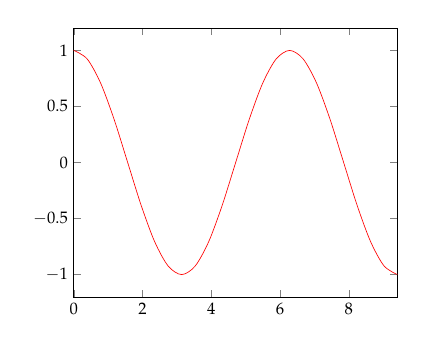
\begin{tikzpicture}[scale=0.60]
		\begin{axis}[xmin=0,xmax=9.42]
		\addplot[color=red,smooth,domain=0:9.42]{sin(deg(x)+90)};
		\end{axis}
	\end{tikzpicture}
	\subcaption{Snake's position at t=1.}
	\end{subfigure}%
	\begin{subfigure}[t]{0.33\linewidth}
	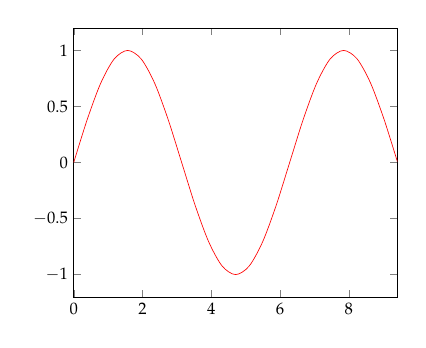
\begin{tikzpicture}[scale=0.60]
		\begin{axis}[xmin=0, xmax=9.42]
		\addplot[color=red,smooth,domain=0:9.42]{sin(deg(x))};
		\end{axis}
	\end{tikzpicture}
	\subcaption{Snake's position at t=2.}
	\end{subfigure}%
	\begin{subfigure}[t]{0.33\linewidth}
	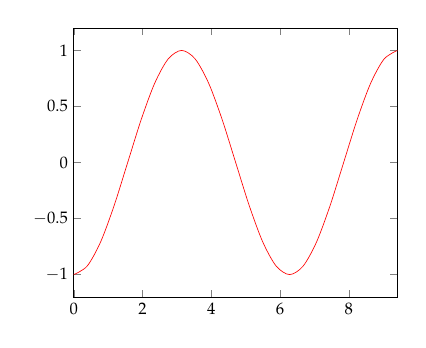
\begin{tikzpicture}[scale=0.60]
		\begin{axis}[xmin=0, xmax=9.42]
		\addplot[color=red,smooth,domain=0:9.42]{sin(deg(x)-90)};
		\end{axis}
	\end{tikzpicture}
	\subcaption{Snake's position at t=3.}
	\end{subfigure}
	\caption{The progression of snake's movement over time represented by variations of a standard \(y=\sin(x)\) graph.}
\end{figure}
The main module determines which direction to curve each segment (or leave in neutral state) with the function \(y=A\sin(B\times x - C) + D\) \cite{Luo2020Motion, Wan2023Design, Luo2018OriSnake}. \(A\) is the amplitude of the function, in this case, it is proportional to how wave the snake curves. \(B\) is the frequency of the function, that is, how horizontally compressed the function is, a larger \(B\) value means more curves in the same length of the robot. \(D\) is neglected in this function because it does affect the direction of travel. \(C\) is the horizontal shift of the function. In the case of the robot, this value is unique to each segment in order for the snake to move like a sine function. Each segment is slight offset to the right of the previous segment, which means that the segment will follow the motion of the previous. Thus, when all segments are combined, the snake forms a moving sine function. Because \(y=\sin(x)\) is a periodic function with a period of 2\(\pi\)/\(Speed\), the value of \(rads\) cycles through 0\degree to 360\degree . In the context of this code, the sine function is as follows. 

\centerline{\(k = \sin(Speed \times rads + id \times shift)\)}Upon receiving a new \(rads\) value from the main module, each segment will calculate its own \(k\) value and perform the corresponding action depending on the value. I evenly divided the function into three parts; if \(k\) is within 1/6 and 1/2, the segment turns left; if it is within -1/6 and -1/2, the segment turns right; otherwise it stays neutral. When staying neutral, the segment will unpower all solenoid valves to release all chambers and have the silicon part return to neutral position. If the segment is turning left, the top and right solenoid valve will close and those two chambers will inflate, making the segment curve to the left. Similarly, if the segment is turning right, the top and left solenoid valve will close so the segment curves to the right. 


\begin{figure} [H]
	\centering
	\begin{subfigure}[t]{0.33\linewidth}
	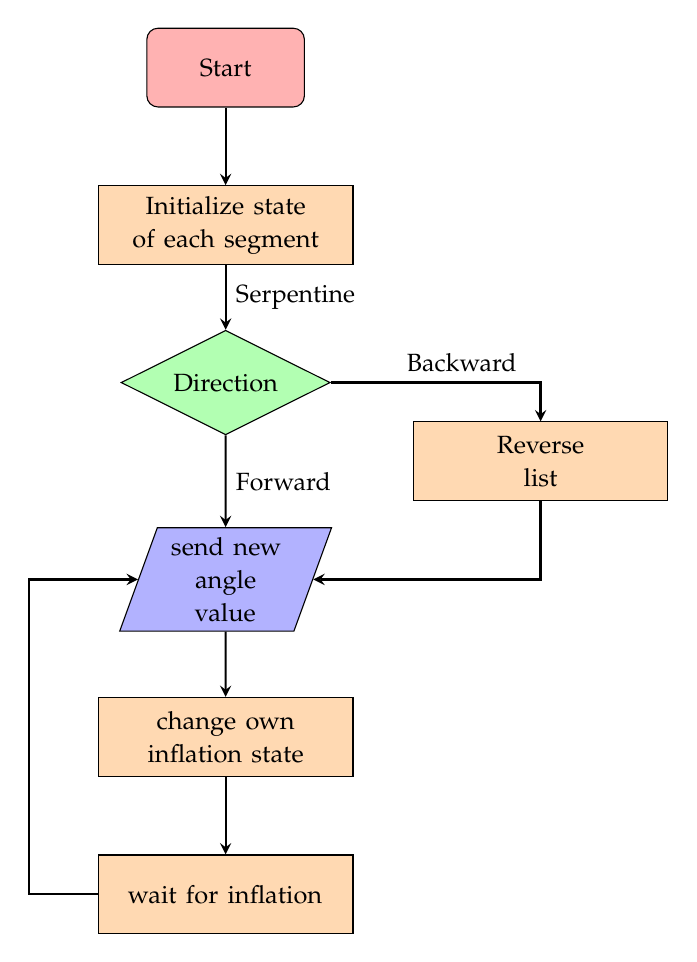
\begin{tikzpicture}[node distance=2cm, auto]
		\node (start) [startstop] {\small Start};
		\node (pro1) [process, below of=start] {\small Initialize state of each segment};
		\node (dec2b) [decision, below of=pro1, yshift=0cm] {\small Direction};
		\node (dec2bb) [process, right of=dec2b, node distance=4cm, yshift=-1cm]{\small Reverse\\ list};
		\node (pro2ba) [io, below of=dec2b, yshift = -0.5cm]{\small send new angle value};
		\node (pro3ba) [process, below of=pro2ba]{\small change own inflation state};
		\node (pro4ba) [process, below of=pro3ba]{\small wait for inflation};
	
		\draw [arrow] (start) -- (pro1);
		\draw [arrow] (pro1) -- node[anchor=west] {\small Serpentine} (dec2b);
		\draw [arrow] (dec2b) -- node[anchor=west] {\small Forward} (pro2ba);
		\draw [arrow] (dec2b) -| node[anchor=south, xshift=-1cm] {\small Backward} (dec2bb);
		\draw [arrow] (dec2bb) |- (pro2ba);
		\draw [arrow] (pro2ba) -- (pro3ba);
		\draw [arrow] (pro3ba) -- (pro4ba);
	
		\node (c1) [coord, on grid, left of=pro4ba, node distance=1.5cm, xshift=-1cm] {};
		\draw [arrow] (pro4ba) -- (c1) |- (pro2ba);
	\end{tikzpicture}
	\caption{Flow chart how the front ESP32CAM commands each segment}
	\end{subfigure}
	\begin{subfigure}[t]{0.66\linewidth}
	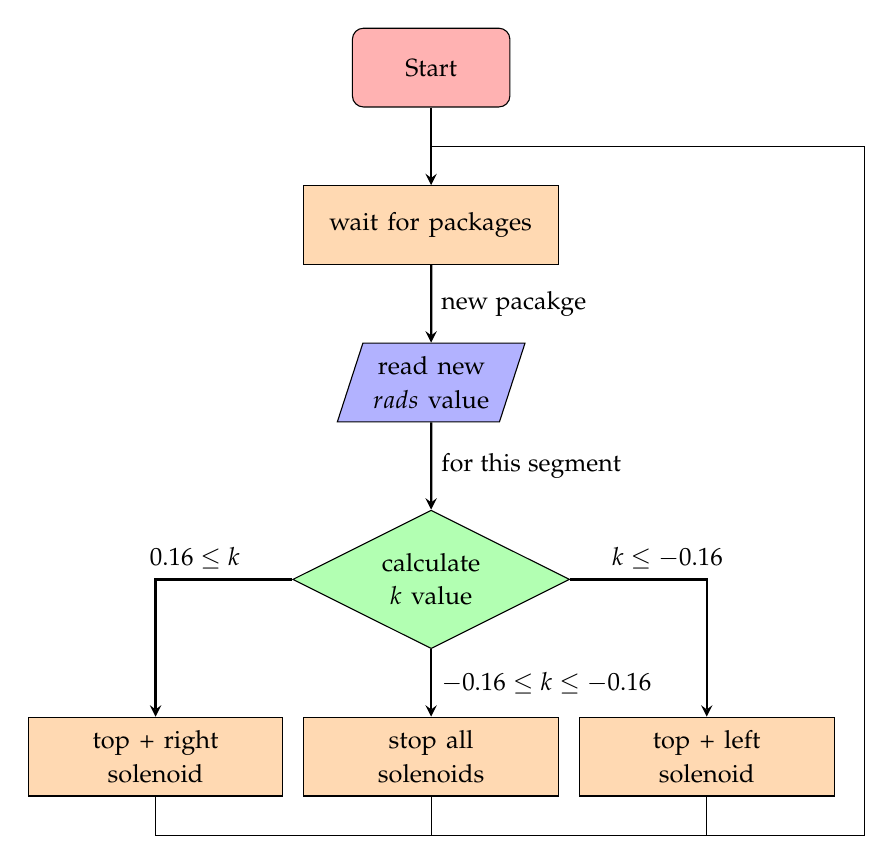
\begin{tikzpicture} [node distance=2cm, auto]
		\node (start) [startstop, xshift=8cm] {\small Start};
		\node (dec1) [process, below of=start] {\small wait for packages};
		\node (dec2) [io, below of=dec1] {\small read new \(rads\) value};
		\node (dec3) [decision, below of=dec2, yshift=-0.5cm] {\small calculate \(k\) value};
		\node (pro4a) [process, below of=dec3, node distance=2.25cm] {\small stop all\\ solenoids};
		\node (pro4b) [process, left of=pro4a, node distance=3.5cm] {\small top + right\\ solenoid};
		\node (pro4c) [process, right of=pro4a, node distance=3.5cm] {\small top + left\\ solenoid};
		\draw [arrow] (start) -- (dec1);
		\draw [arrow] (dec1) -- node {\small new pacakge} (dec2);
		\draw [arrow] (dec2) -- node {\small for this segment} (dec3);
		\draw [arrow] (dec3) -- node {\small \(-0.16 \le k \le -0.16\)} (pro4a);
		\draw [arrow] (dec3) -| node[anchor=south, xshift=0.5cm] {\small \(0.16 \le k\)} (pro4b);
		\draw [arrow] (dec3) -| node[anchor=south, xshift=-0.5cm] {\small \(k \le -0.16\)} (pro4c);
		\node (c1) [coord, on grid, right of=dec1, xshift=1cm] {};
		\node (c2) [coord, on grid, below of=pro4c, xshift=2cm, yshift=1cm] {};
		\node (c3) [coord, on grid, above of=dec1, yshift=-1cm] {};
		\draw (pro4b) |- (c2) |- (c3);
		\draw (pro4a) |- (c2) |- (c3);
		\draw (pro4c) |- (c2) |- (c3);
	\end{tikzpicture}
	\caption{Flow chart of how each segment functions}
	\end{subfigure}
\end{figure}

\subsection{Remote Control and Video Stream}
The phone app was made with the AppInventor from MIT. In order to send video stream to and receive controls from the phone, a TCP connection was established between the phone and the front esp32cam module. The esp32cam module served as a web server and the phone connected to it through HTTP protocol. The phone app is a framed web page and commands were sent through this connection using GET. The video stream was also pulled from the web server through http as well. 
\begin{figure} [H]
\centering
	\includegraphics[width=0.5\linewidth]{appinventor}
	\caption{Screenshot of the AppInventor Page}
\end{figure}

\begin{figure} [H]
\centering
	\includegraphics[width=0.2\linewidth]{video stream}
	\caption{Screenshot of the app}
\end{figure}


\section{Tests}
\subsection{Single Segment Test}
I first tested the performance of a single segment in real life. The first test was unsuccessful as even the solenoid valves didn't open when powered. Normally, the solenoid valve would have a "click" sound when it is powered and unpowered. I also checked the power source, which outputs 12V and I've stepped it down to little more than 6V. After check the voltage at different points, I concluded that when the current passed through the A4950 driver, a 5V current is outputted rather than the 6V input. It seems like the voltage would drop significantly after passing through A4950 until the input is around 8V, which is when the voltage drop stops and outputs the same voltage as input. After dialing the power input to 8V, the solenoid valves now work.
\begin{table} [H]
	\centering
	\begin{tabular}{|c|c|c|c|}
	\hline
	Time (s) & 1 & 2 & 3\\
	\hline
	$\Delta$x (cm) & 1.57 & 2.67 & 3.52\\
	\hline
	Image & \includegraphics[align=c, scale=0.2]{1} & \includegraphics[align=c, scale=0.2]{2} & \includegraphics[align=c, scale=0.2]{3}\\
	\hline
	\end{tabular}
	\caption{Screenshots of the segment inflating}
\end{table}
I filmed an top-down video of the first segment of the snake inflating and then imported into the software called Tracker from physlets.org to collect the data from the video. I first imported the video into the software. Then, I added a coordinate axis and aligned the y-axis along the snake. Measuring that the distance between the wheels of different segments to be 0.116 meters, I added a calibration stick to set the reference. Then I added a point mass tracking point and ran the autotracker. After testing, I plotted the x position relative to the time and the trend seems to be logarithmic. The maximum distance is 3.62cm at t=3.44s.
\begin{figure} [H]
\centering
\includegraphics[width=0.8\textwidth]{single seg}
\caption{x position of the point relative to time}
\end{figure}

\subsection{Two Segment Test}
Similar to the single segment test, I filmed an top-down video of the first segment of the snake inflating and then followed the same steps as I've previously done. After testing, I plotted the x position relative to the time and the trend seems to be logarithmic. The maximum distance is 11.25cm at t=3.60s.

\begin{table} [H]
	\centering
	\begin{tabular}{|c|c|c|c|}
	\hline
	Time (s) & 1 & 2 & 3\\
	\hline
	$\Delta$x (cm) & 3.66 & 8.39 & 10.33\\
	\hline
	Image & \includegraphics[align=c, scale=0.2]{11} & \includegraphics[align=c, scale=0.2]{22} & \includegraphics[align=c, scale=0.2]{33}\\
	\hline
	\end{tabular}
	\caption{Screenshots of the segment inflating}
\end{table}
\begin{figure} [H]
\centering
\includegraphics[width=0.8\textwidth]{two seg}
\caption{x position of the point relative to time}
\end{figure}

\subsection{First Version Wheel Speed Test}

For this test, I followed similar procedures as the previous tests and used wheels from the first version. The snake traveled 10.05cm in 14.74s with a speed of 0.68cm/s. The most likely cause of the decrease in rate after t=20s is due to the distortion of the video as it is now filming the snake at an angle. 

\begin{table} [H]
	\centering
	\begin{tabular}{|c|c|c|c|c|}
	\hline
	Time (s) & 5 & 10 & 15 & 20\\
	\hline
	$\Delta$x (cm) & 4.39 & 7.51 & 10.57 & 13.43\\
	\hline
	Image & \includegraphics[align=c, scale=0.2]{5} & \includegraphics[align=c, scale=0.2]{10} & \includegraphics[align=c, scale=0.2]{15} & \includegraphics[align=c, scale=0.2]{20}\\
	\hline
	\end{tabular}
	\caption{Screenshots of the segment in motion}
\end{table}

\begin{figure} [H]
\centering
\includegraphics[width=0.8\textwidth]{4 seg snake}
\caption{Distance traveled by the snake over time}
\end{figure}
\subsection{Final Version Wheel Speed Test}

I also ran the same test with the final version of the wheel to better compare the two versions. For this test, I followed the same procedures as the previous tests with the latest version of wheels. The snake traveled 33.07cm in 14.73s with a speed of 2.25cm/s. This is 331\% ($\frac{2.25cm/s}{0.68m/s}=3.31$) of the speed of the first version.

\begin{table} [H]
	\centering
	\begin{tabular}{|c|c|c|c|c|}
	\hline
	Time (s) & 5 & 10 & 15 & 20\\
	\hline
	$\Delta$x (cm) & 11.09 & 22.12 & 33.72 & 43.41\\
	\hline
	Image & \includegraphics[align=c, scale=0.2, angle=90]{5_2} & \includegraphics[align=c, scale=0.2, angle=90]{10_2} & \includegraphics[align=c, scale=0.2, angle=90]{15_2} & \includegraphics[align=c, scale=0.2, angle=90]{20_2}\\
	\hline
	\end{tabular}
	\caption{Screenshots of the segment in motion}
\end{table}

\begin{figure} [H]
\centering
\includegraphics[width=0.8\textwidth]{full_snake_improve}
\caption{Distance traveled by the snake over time}
\end{figure}

\section{Conclusion}

During this project, the basic functionalities of a robotic snake has been achieved. An improved mold for the silicone body was designed, and the idea of using detachable inner pillars can be implemented elsewhere as well in similar situations where an airtight seal was required. This single-opening silicone silicone design with an air valve minimized the chance of leakage. To find the optimal parameters, physics simulations were ran to determine the best wall thickness and diameter of the silicone part. The modularity of snake segments was also achieved with independent control units and the I2C protocol, which allows for multiple connection using the same bus. The basic functionality of video stream and remote control has also been achieved. Finally, to test the finished product, two sets of test were performed and measurements were taken. 

However, this project did not achieve everything planned at the beginning. It only achieved the basic function of the robot, yet it is lacking a lot of software to support it. The implementation of an AI image recognition system is crucial as well as a purely image-based mapping system is also yet to be done. A coordinate system is also necessary to know the actual location of the snake. Without these, the robot cannot achieve its full potential as a life-saving device. Apart from the software, the silicon body design will also need to be improved as the current design does not make use of the pull potential of the air pressure. The movement algorithm can also be improved as right now the robot moves rather slowly.





%----------------------------------------------------------------------------------------
%	REFERENCE LIST
%----------------------------------------------------------------------------------------
\newpage	
\printbibliography

%----------------------------------------------------------------------------------------

\end{document}
